\setcounter{chapter}{3}
\setcounter{section}{0}
\setcounter{figure}{0}
\setcounter{equation}{0}
\setcounter{table}{0}
\chapter*{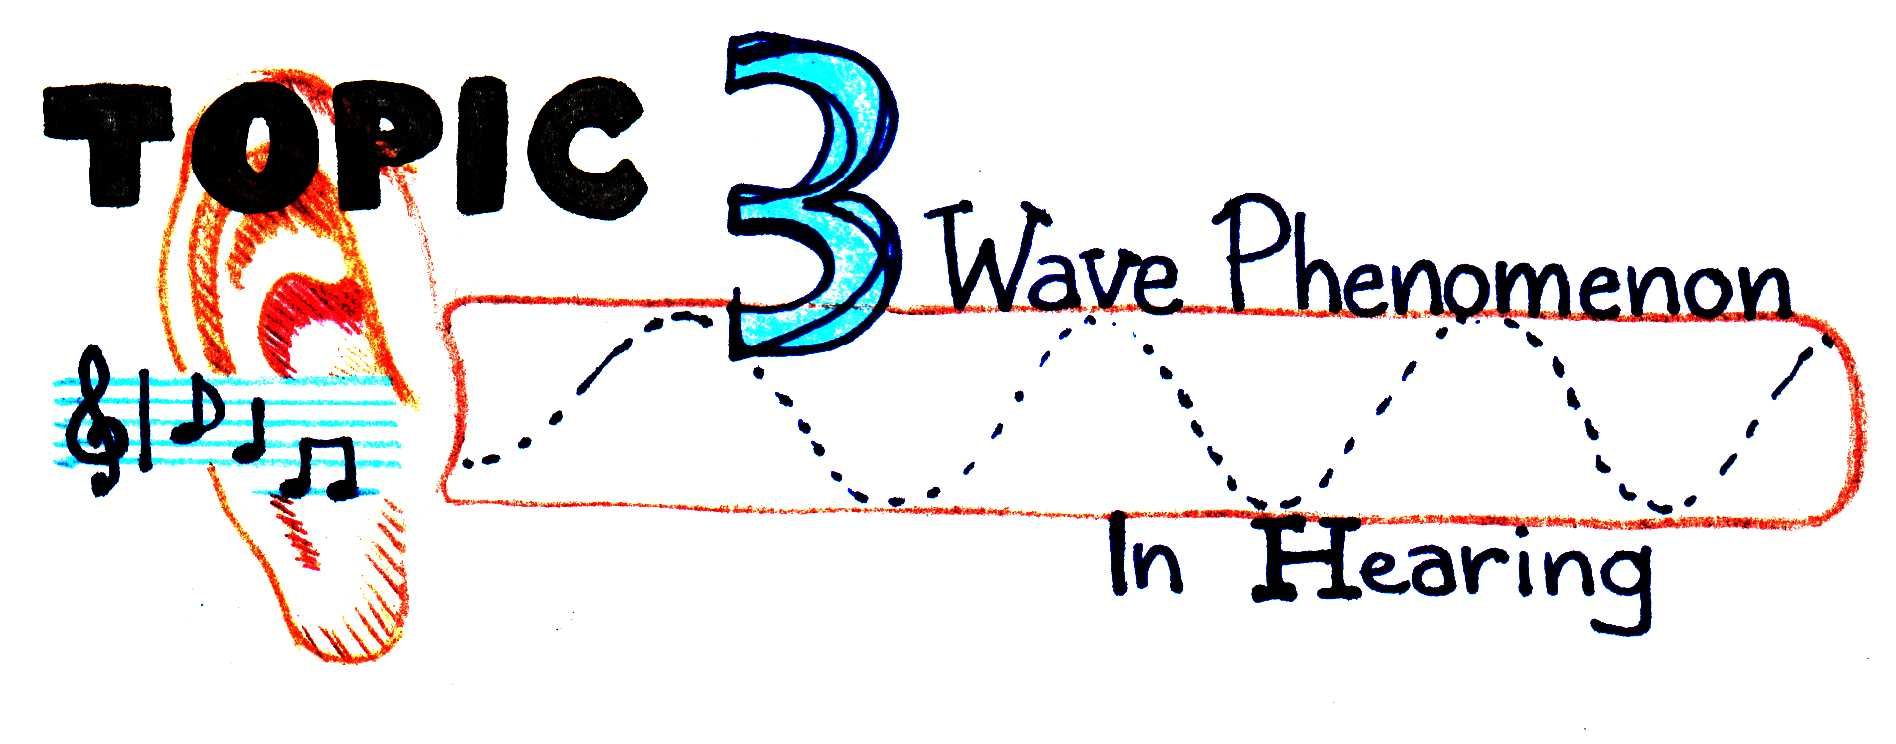
\includegraphics[width=\textwidth]{./figures/Topic3/Topic3.jpg}}
\addcontentsline{toc}{chapter}{Topic 3: Wave Phenomenon in Hearing}

\section{Introduction}

The human ear can detect an extraordinary range of sound intensities, from a faint whisper to a clap of thunder 10 billion times as loud.  The ear can also distinguish frequencies from 20 to 20,000 Hz, allowing us to pick a familiar voice out of a crowd or enjoy the nuances of an aria.  How does the ear perceive such a wide range of sounds, and how is the information transmitted to and integrated in the brain?  
In this chapter, we will first review the physical properties of sound waves and then explore how the ear functions in terms of them.

\section{General Properties of Sound Waves and Hearing}

Sound is a pressure wave traveling in a medium.  We normally consider the medium to be air, but sound travels through liquids and solids as well.  For humans, as noted in the Introduction, the audible range is 20-20,000 cycles per second (Hertz).  Our hearing is particularly well suited to frequencies near 3,700 Hz, which corresponds to human speech.  
\begin{figure}[htb]
	\centering
	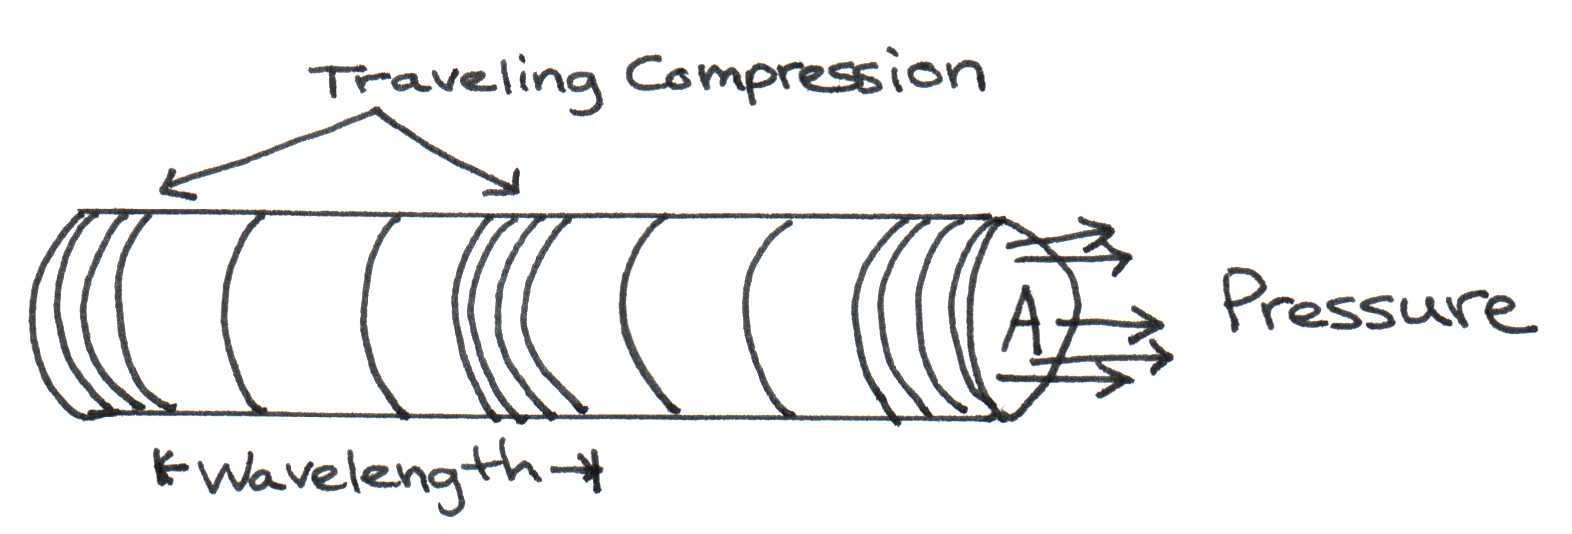
\includegraphics[width=\textwidth]{./figures/Topic3/Fig3-1.jpg}
	\caption{Moving pressure differences.}
	\label{Fig3-1}
\end{figure}
Energy is carried by sound waves in the form of moving pressure differences.  It is important to note that molecules of the medium do not travel the length of the medium with the energy—they transmit the energy by vibrating.   Think of the molecules as a line of people passing along slices of birthday cake at a party.  While the people (the medium) move slightly to do the passing, it is the cake (the energy) that is carried across the room.  For a more accurate analogy of how sound waves propagate, imagine that the medium acts as a slinky.  When the slinky is stretched out, you can create a wave by pinching several rings together at one end and releasing them.  The compression moves along the length of the slinky with a constant speed, c.  As the compression moves past a certain point, energy causes the ring at that point to become displaced by a certain amount in the direction of the wave.  However, the ring stays in the same position relative to the other rings, so only the energy is transmitted.  Similarly, air molecules are pushed together as a sound wave passes, creating a pocket of higher pressure between areas of lower pressure.  It is this compression that gets passed along to adjacent molecules.  Each atom vibrates sinusoidally with a velocity
\begin{equation}\label{eqn3-1}
v(t) = v_o \sin\left(\omega t\right)
\end{equation}
where $v_{\circ}$ is the amplitude of the  velocity of the atom and $\omega$ is its angular frequency, equal to $2\pi$ times the frequency, $f$.  The velocity of an atom, $v$, is not to be confused with the velocity of the wave, c. The speed of sound in air is constant through an air mass of uniform temperature.  We will use c = 350 m/s, which is equivalent to 785 mph.  

The intensity of a sound wave depends on the amount of energy it carries and is related to loudness.  Specifically, intensity measures the work done by the pressure wave per unit time on a surface of area $A$.  Recall that work is the product of force and distance.  If $\Delta x$ is the displacement of a molecule in time period $\Delta t$, then the intensity is
$${\rm Intensity} = \frac{\rm Work~done~by~pressure}{{\rm Area}\cdot{\rm time}}$$
$$I = \frac{W}{A \cdot\Delta t}$$
$$I = \frac{F\cdot \Delta x}{A\cdot t}$$
and since force divided by area is pressure, and $\Delta x$ divided by $\Delta t$ is velocity
\begin{equation}\label{eqn3-2}
I = P v
\end{equation}
where $P$ is the instantaneous pressure as the sound wave passes by, and $v$ is the instantaneous velocity of the atoms driven into oscillation by the pressure.  The magnitude of $P$ is directly related to magnitude of the velocity $v$ of the atoms in the neighboring layer. In fact,
\begin{equation}\label{eqn3-3}
P=\mathcal{Z} v
\end{equation}       

One might expect that lighter atoms/molecules might achieve greater velocities when pushed by the same pressure. Hence the constant $\mathcal{Z}$, which is known as the impedance, must be related to inertia (mass) of the medium. In fact, it can be shown to be the product of the density of the medium, $\rho$, the speed of the sound wave, c, and the area affected sound, $A$.    
\begin{equation}\label{eqn3-4}
\mathcal{Z} = \rho c A
\end{equation}
The concept of impedance is central toward understanding what fraction of sound gets transmitted across the eardrum and into the brain.  We will discuss how this works in a later section.

Sound intensity is sometimes measured in Watts/m$^2$ or Watts/cm$^2$.  The threshold of hearing is approximately 10$^{-12}$ Watts/cm$^2$.  This intensity corresponds to the sound that a mosquito produces several meters away from your ear. To give you another idea of how faint this intensity is, this is equivalent to the intensity of light originating from a 100 Watt incandescent light bulb falling on a 1 cm$^2$ target placed 500 miles away!  At the upper end of the threshold spectrum, the ear detects signals up to 10$^{-6}$ Watts/cm$^2$. The maximum intensity a person can withstand is approximately 100 dB or 10$^{-2}$W/m$^2$.
 
Because the audible range covers ten orders of magnitude, sound is quantified on a logarithmic scale (base 10) rather than on a linear one. See Fig.~\ref{decibels}.
\begin{figure}[htb]
	\centering
	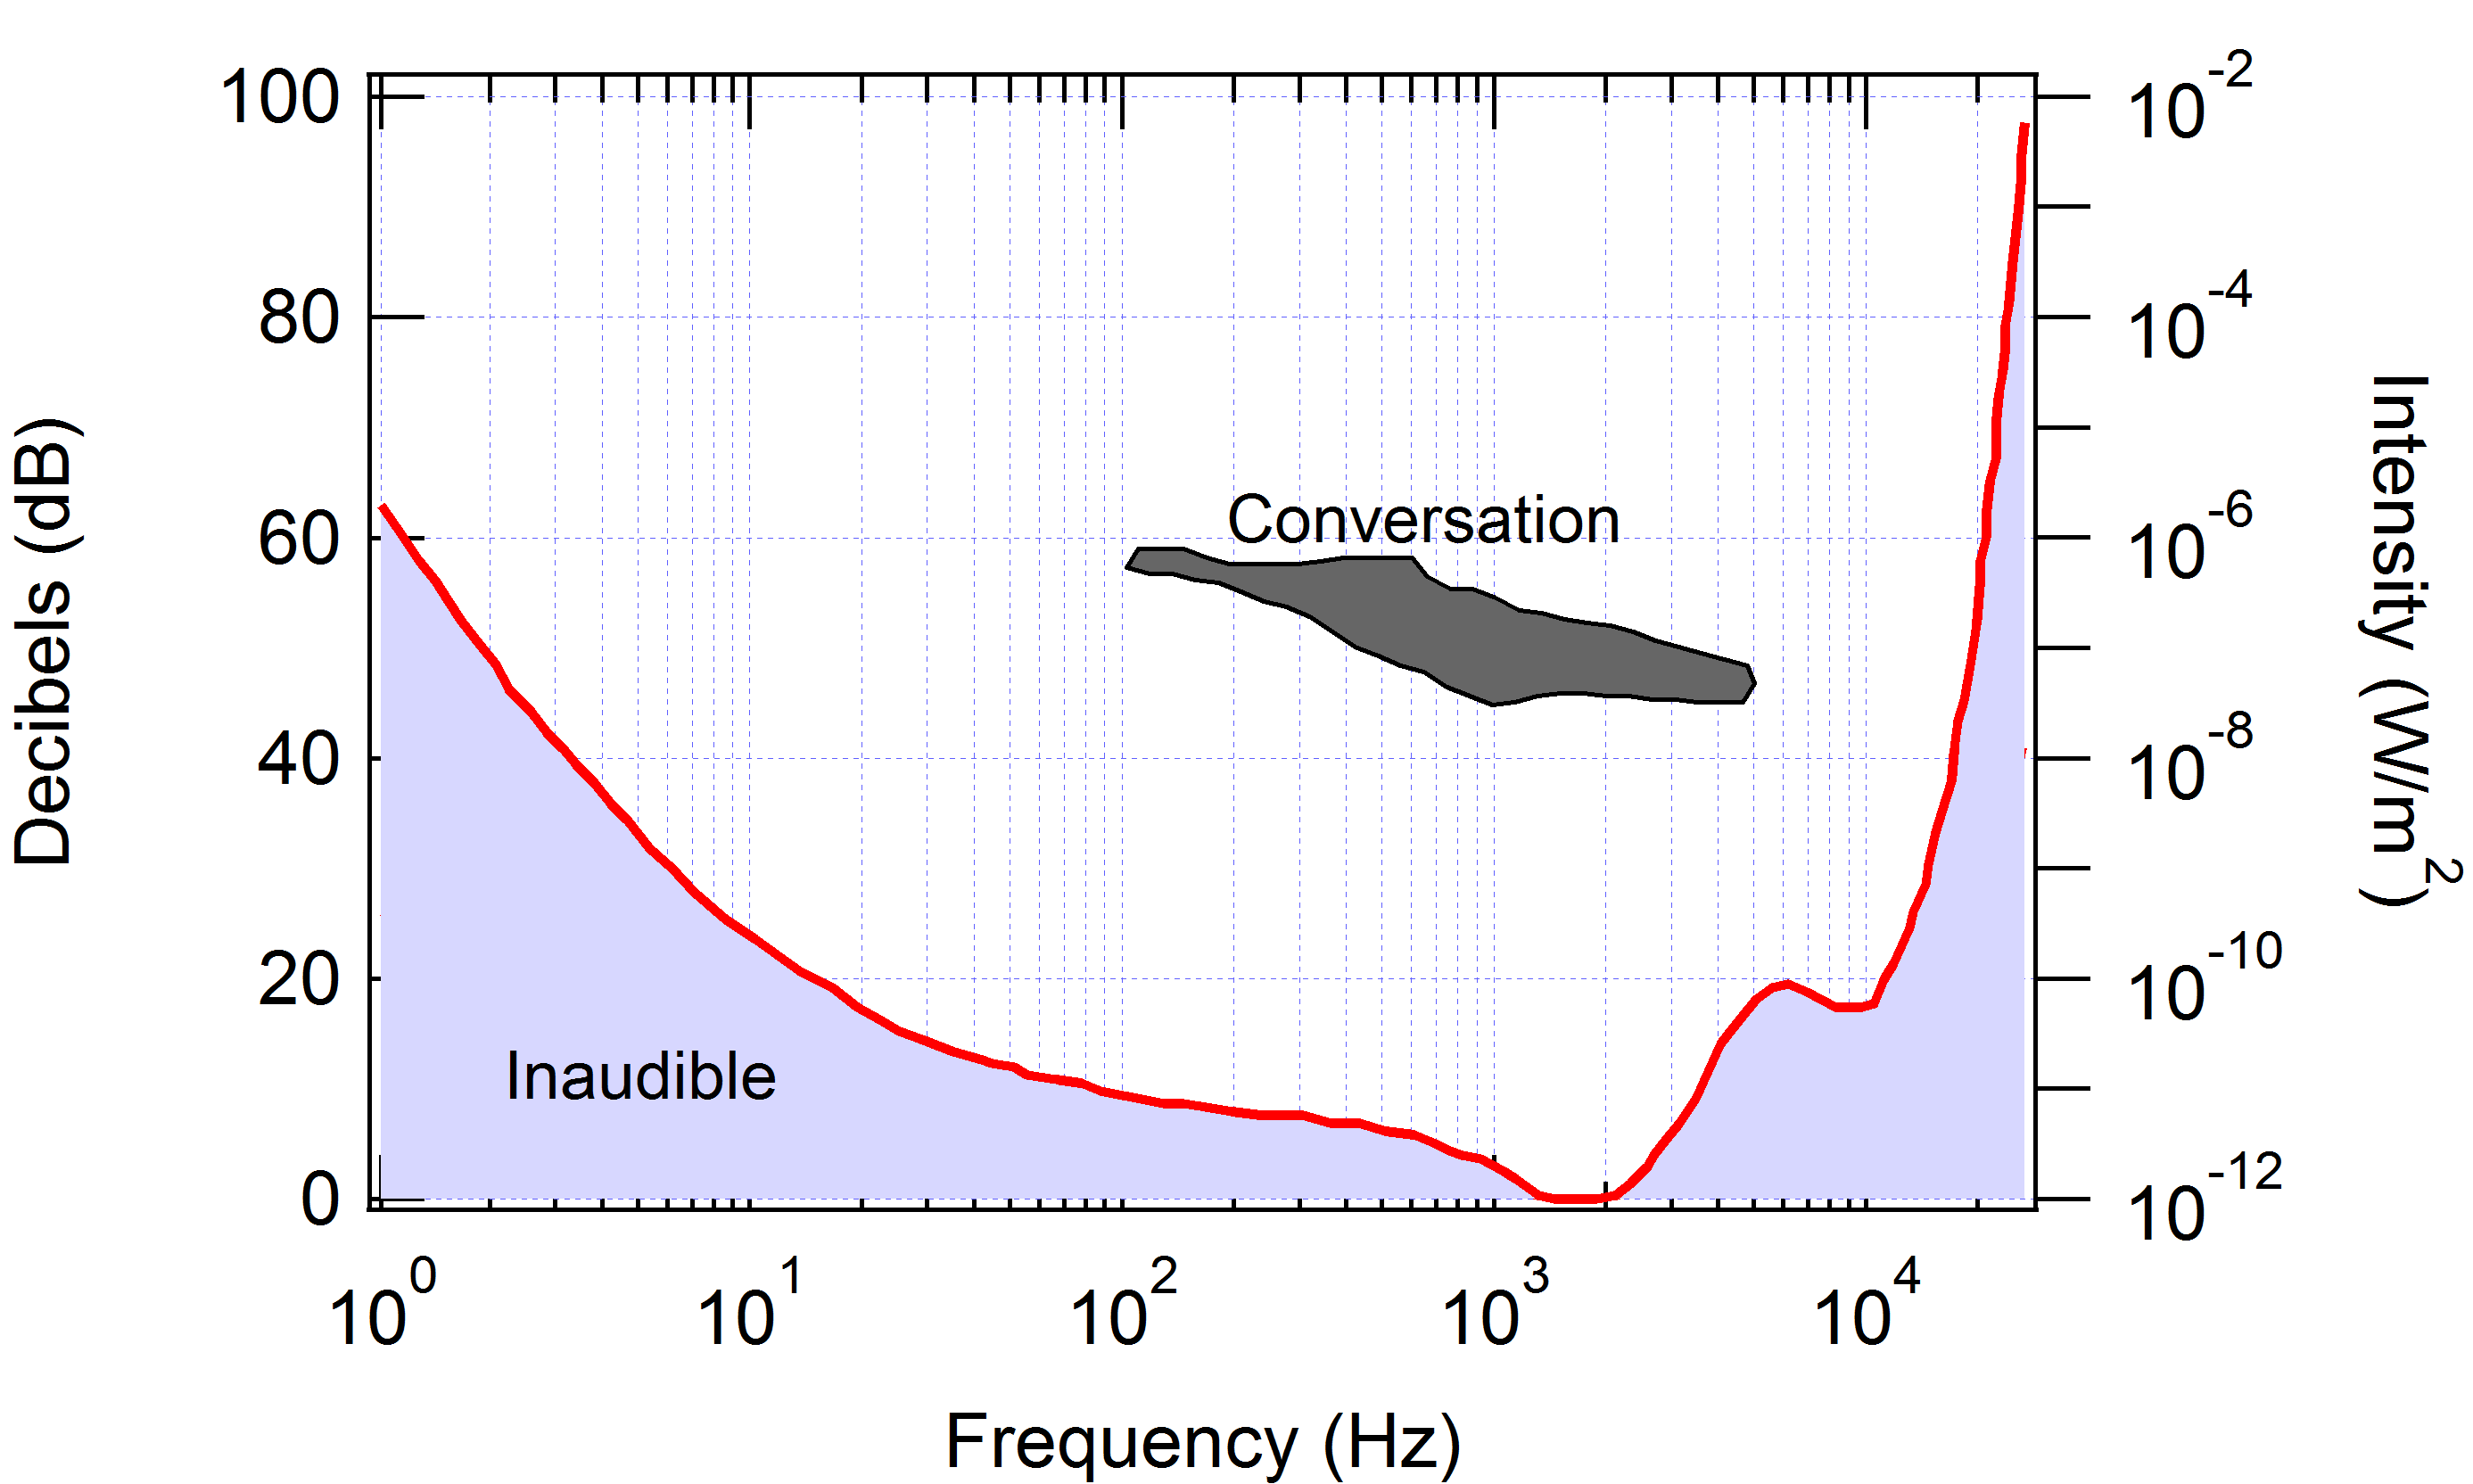
\includegraphics[width=4.5in]{./figures/Topic3/Fig3-decibels.png}
	\caption{Audible threshold vs. frequency. Conversational intensity is shown shaded in the central region of the graph. The lowest audible decibel level is 0 ($I=10^{-12}$W/m$^2$), which occurs at about 2500 Hz.}
	\label{decibels}
\end{figure}
According to this scale, every change in intensity by a factor of ten above some reference level is called a bel.  Usually, the reference level is taken to be the threshold of sound, 10$^{-12}$ W/cm$^2$.  Accordingly, the number of bels for a sound with intensity $I$ relative to this reference level is $\log_{10}\left(I/10^{-12}\right)$.  Often in acoustics, the bel scale is too coarse to quantify loudness.  For this reason, a finer unit is used -- the decibel -- where 1 bel = 10 decibels.  Therefore the sound intensity level in decibels is quantified by the formula
\begin{equation}\label{eqn3-5}
{\rm dB~level} = 10 \log_{10}\left(\frac{I}{10^{-12}}\right)
\end{equation}
Using this scale, one can quantify sound loudness for several sources such as those listed in Table \ref{decibel-table}.
\begin{table}[h]
\begin{center}
\begin{tabular}{|l|c|}
\hline
Source & Loudness (dB) \\
\hline
Whisper & 20--30 \\
Normal conversation & 60--70 \\
Leaf blower near user & 100--110 \\
\hline
\end{tabular}
\caption{Intensity levels in decibels for several common sources of sound.}
\label{decibel-table}
\end{center}
\end{table}

It should be noted that the decibel scale is also used for characterizing changes relative to some arbitrary initial level, i.e. something other than the threshold of hearing. For example, if the sound intensity level is known to increase from some initial level to a final level that is 1000 larger, then one can say that the intensity level increased by 
\begin{eqnarray}\label{eqn3-6}
{\rm dB~change} &=& 10 \log_{10}\left(\frac{I_{\rm final}}{I_{\rm initial}}\right)\\
&=& 10 \log_{10}(1000)\nonumber\\
&=& 30~{\rm dB}\nonumber
\end{eqnarray}

\section{Structure and Function of the Ear}
 
The ear can be divided into three modules (Fig.~\ref{Fig3-2}), each of which performs an important function based on physical principles.  The ear canal, also known as the auditory canal or outer ear, collects sound waves from air and funnels them to the sound-sensing apparatus deep inside the head.  The ear canal, because of its tubular shape, acts as a resonator that allows the ear to hear sound frequencies within the resonance range better than others.  The second module, the middle ear, is designed to increase the transmission of sound waves as they pass from the air to the aqueous fluid of the inner ear, the third module.  The inner ear, in turn, contains sensors that convert water waves into nerve impulses.  The following sections describe the physical principles behind these functions. 
\begin{figure}[h]
	\centering
	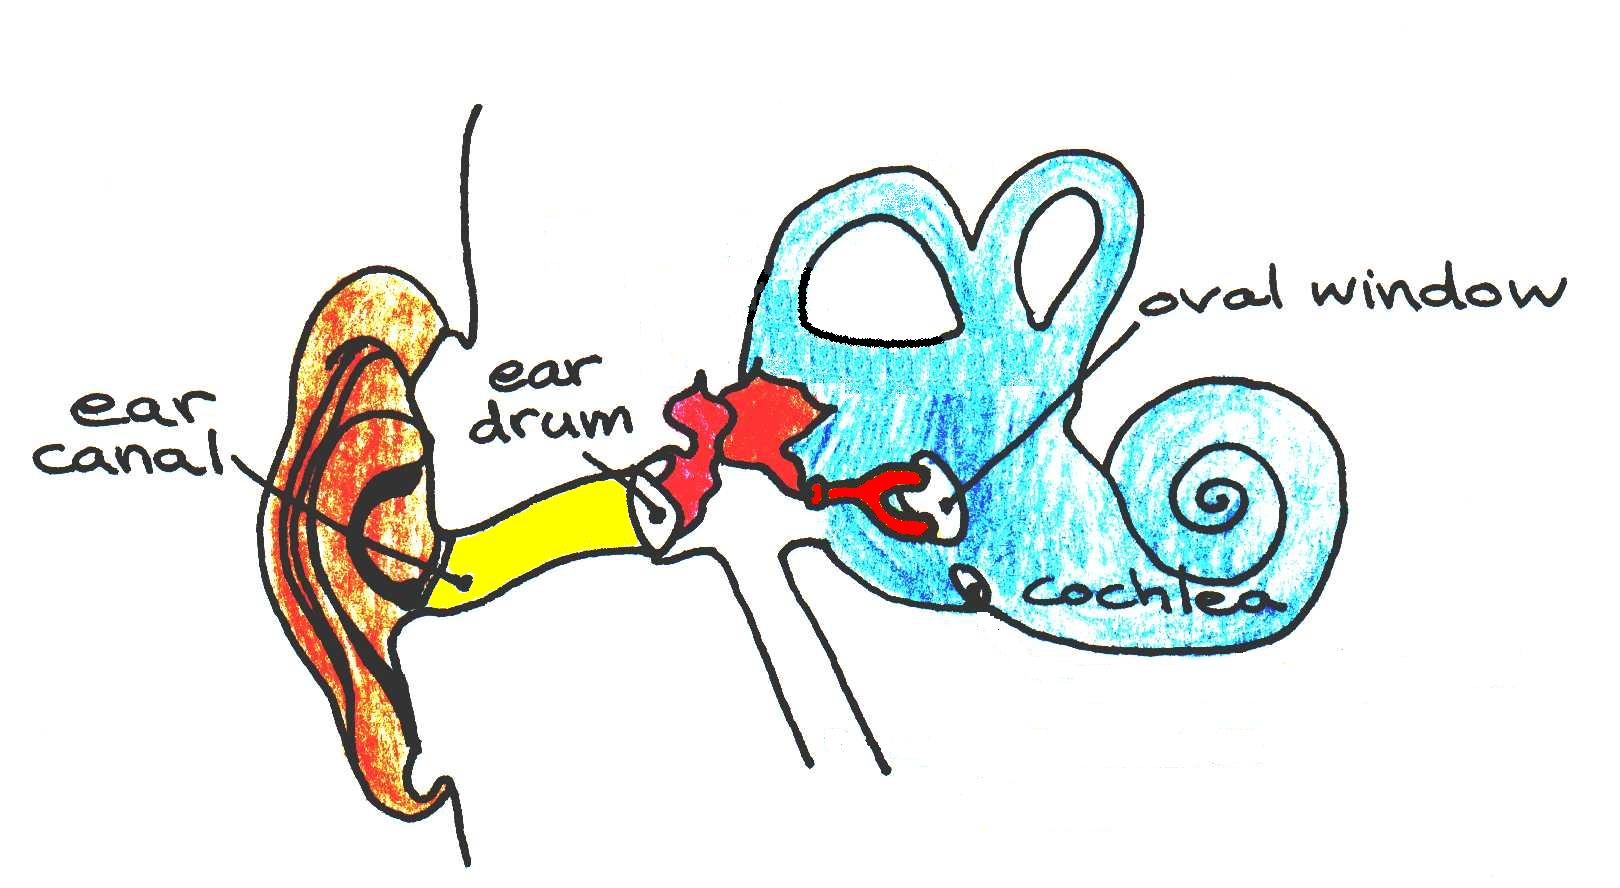
\includegraphics[width=\textwidth]{./figures/Topic3/Fig3-2.jpg}
	\caption{Cross-section of the human ear. The regions filled in yellow, red, and blue correspond to the outer ear (ear canal), the middle ear, and the inner year, respectively.}
 	\label{Fig3-2}
\end{figure}

\subsection{The Auditory Canal}

The outer ear acts as a filter, restricting the passage of certain frequencies to the inner ear.  This performance can be understood in terms of acoustical resonances.  Before proceeding with our discussion, we will first review the principles behind the resonance phenomenon for both closed and opened pipes. Although the closed end case is not pertinent to the discussion of hearing, the equation developed will be useful for a forthcoming discussion of electron resonances within molecules (Topic 6).

\subsubsection{Resonance in a Closed Pipe}

At the closed ends of a pipe, air molecules are unable to vibrate since their motion is blocked by the obstruction that seals the pipe.  Those regions and others where the air does not move are called displacement nodes.  Regions where the pressure does not change are called pressure nodes. In acoustical waves, the displacement is out of step with pressure these regions must correspond to places of maximum pressure. These places are known as pressure anti-nodes.  As you might guess, regions where air molecules move the greatest distance are called displacement anti-nodes.  These points correspond to areas of minimum pressure and are thus also called pressure nodes.  Henceforth, when we speak of nodes and anti-nodes, we will be referring to displacement nodes and anti-nodes, unless otherwise indicated.  

\begin{figure}[htb]
	\centering
	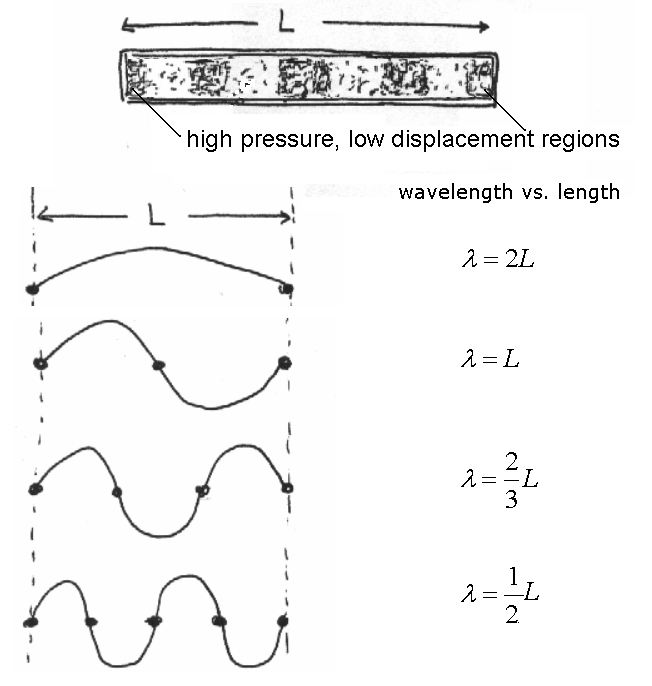
\includegraphics[width=5.0in]{./figures/Topic3/Fig3-3.png}
	\caption{Acoustic patterns inside close-ended pipes.}
 	\label{Fig3-3}
\end{figure}
As shown in Fig.~\ref{Fig3-3}, there are several resonances that can occur inside a closed pipe. The first contains only two nodes at each end and a single anti-node in the middle of the pipe.  In this case, only one half of a full wavelength fits in the pipe.  Thus, for a pipe of length $L$, $\lambda = 2L$.  This is known as the first, or the fundamental, resonance.  If the frequency of the wave increases until there are three nodes and two antinodes, one full wavelength fits in the pipe.  Here, $\lambda = L = (2/2)L$.  Similarly, when there are four nodes, there are three antinodes, and one and a half wavelengths fit in the pipe.  The wavelength changes to $\lambda = (2/3)L$.  We could continue in this same manner forever.  In general, 
\begin{equation}\label{eqn3-7}
\lambda = \frac{2L}{n}
\end{equation}
where $n$ is the number of anti-nodes, always an integer $\geq$ 1. 

\subsubsection{Resonance in a Single Open End Pipe}

The ear canal behaves like a pipe open on one end.  As with the closed pipe, air cannot vibrate at the closed end, so it must be a node.  However, air at the open end is at the same pressure as air outside the pipe, so a pressure node, or a displacement anti-node must be located there.  As shown in Fig.~\ref{Fig3-4}, this means that at the fundamental resonance there is only one node and one anti-node in the pipe. Consequently, only one-fourth of a wavelength fits in the pipe and thus $\lambda = (4/1)L$.  The next resonant pattern corresponds to one with two nodes and two anti-nodes, for which three-fourths of a wavelength fit in the pipe and so $\lambda = (4/3)L$. And the general formula for the pattern becomes 
\begin{equation}\label{eqn3-8}
\lambda = \frac{4L}{2n+1},
\end{equation}
where $n$ = 0, 1, 2, ... ($2n+1 = $~odd integers). Figure $3.5$ below shows the pattern.
\begin{figure}[htb]
	\centering
	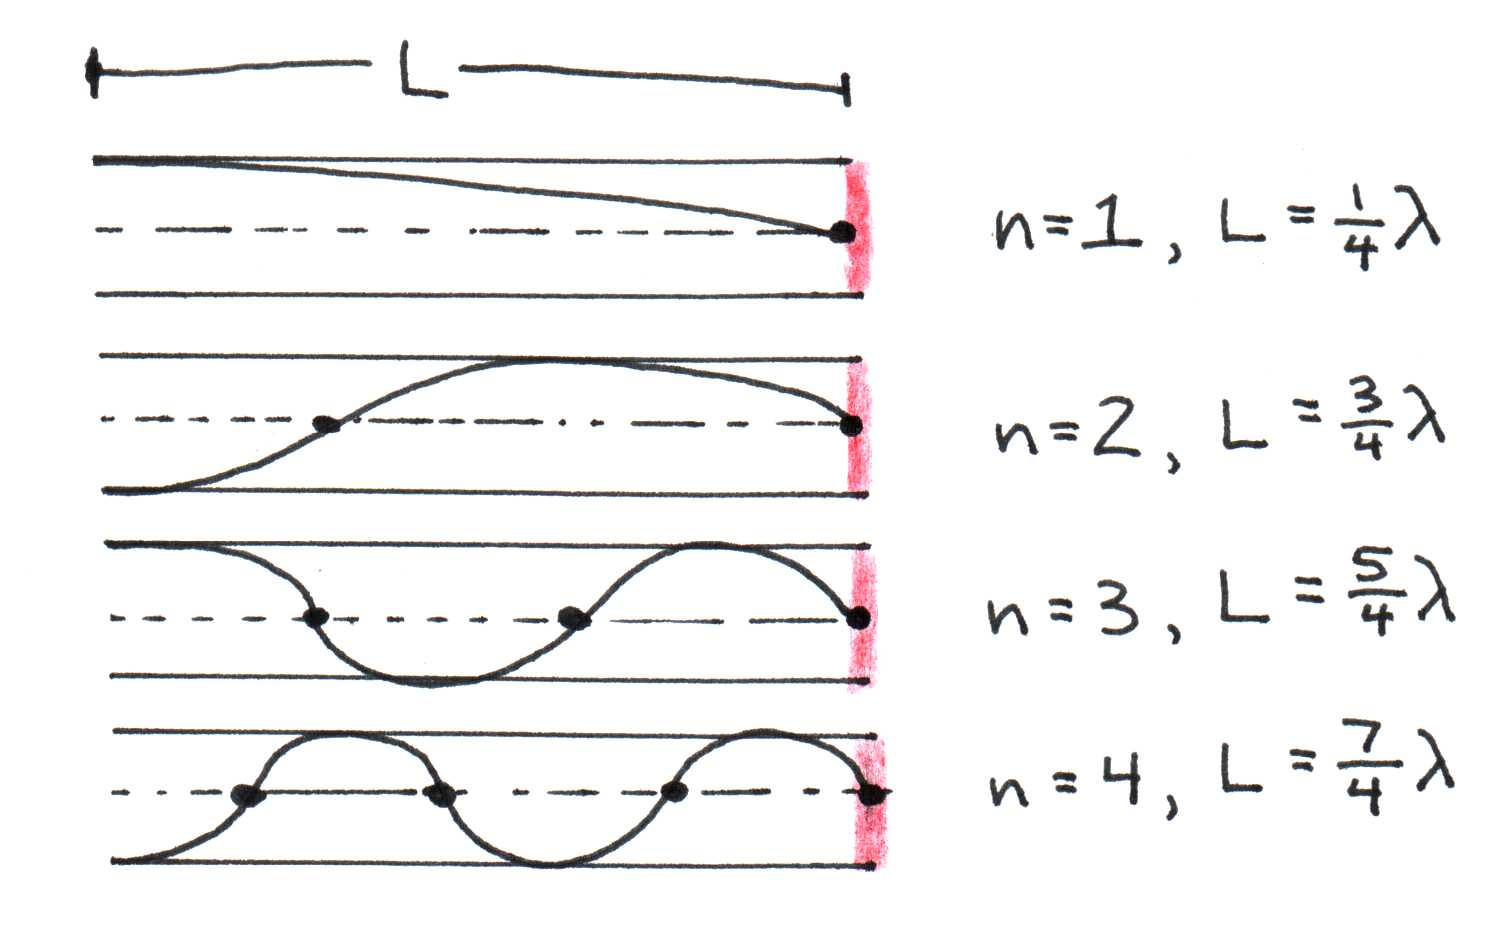
\includegraphics[width=\textwidth]{./figures/Topic3/Fig3-4.jpg}
	\caption{Acoustic resonances in a single open ended pipe.}
	\label{Fig3-4}
\end{figure}
The open-ended pipe model can be used to calculate the resonance frequencies of the human ear.  The lowest frequency at which sound resonates in the ear is found with the above equation where $n$ = 1.  Knowing that c = $\lambda f$, we get c = $4L \cdot f$.  The ear canal is about an inch long, so $L$ = 2.5 cm = 0.025 m.  As noted before, the speed of sound in air is c = 350 m/s.  Using these values, we solve for $f$:
\begin{align}
f &= \frac{c}{4L}\nonumber\\
  &= \frac{350}{4\cdot 0.025}\nonumber\\
  &= 3500~{\rm Hz}\nonumber
\end{align}
In fact, the ear is most sensitive near 3,000 Hz, in agreement with our estimate made above.  The next resonance is predicted to have a frequency three times higher, i.e. 10,500 Hz.  Studies have shown that a small resonance does indeed exist near 12,000 Hz. Notice the increase in sensitivity at this frequency in Fig.~\ref{decibels}. The relation between resonant frequency and the length of the ear canal helps to explain why smaller animals have hearing tuned to higher frequencies, compared to those of larger animals. For instance, the hearing range of mice and rats is between 1000 and 100,000 Hz, while that of an elephant falls between 1 and 20,000Hz.  

\subsection{The Middle Ear}

Sound waves funneled through the auditory canal cause the eardrum to vibrate.  The vibrations are conducted through the three tiny bones (collectively called the ossicles) of the middle ear to their point of contact on the cochlea (inner ear) known as the oval window.  These bones serve two purposes: they protect against loud noises through the attenuation reflex, and they provide what is known as impedance matching between the outer ear and inner ear.  The attenuation reflex occurs when muscles reduce the action of the ossicles in response to a harmfully loud noise.  The physics of impedance matching will be discussed in depth in the following section.

\subsubsection{Impedance Matching}

When sound waves traveling in air collide with the surface of another medium, like water, they are mostly reflected.  Only a fraction of the wave’s energy is transmitted to the target medium.  You might have experienced this while swimming -- if someone tries to speak to you while you are under water, you will be unable to hear the person, because the sound waves bounce off the surface of the pool.  This phenomenon can be explained in terms of the conservation laws of momentum and energy.  Recall from Fig.~\ref{Fig3-1} that it is the pressure changes associated with a sound wave that propels a pocket of molecules to move through the air.  When one of these pockets of air traveling with a velocity $v_{a1}$ collides with a stationary mass of water ($v$ = 0), the collision is essentially elastic, meaning that no kinetic energy is lost.  Some of the air’s kinetic energy is transferred to the water mass, so that the air mass bounces off with velocity $v_{a2}$ and the water mass moves with velocity $v_{w}$.  This is depicted in Figure \ref{Fig3-5} below.
\begin{figure}[htb]
	\centering
	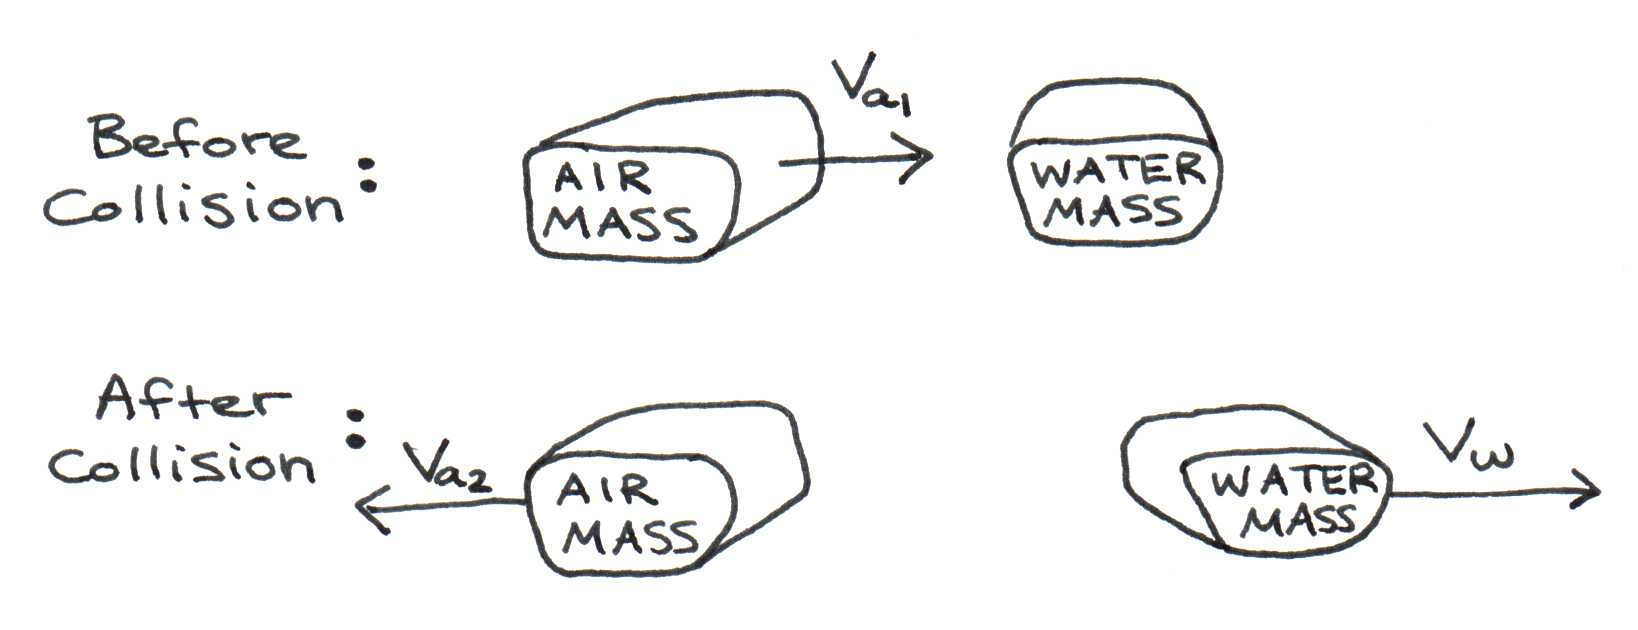
\includegraphics[width=5.0in]{./figures/Topic3/Fig3-5.jpg}
	\caption{Collision of an air mass (pressure pocket) with a stationary water mass.}
 	\label{Fig3-5}
\end{figure}
 
According to the conservation laws,
\begin{align}
m_av_{a1} &= m_av_{a2} + m_wv_w &{\rm Momentum}\nonumber\\
\frac{1}{2}m_av_{a1}^2 &= \frac{1}{2}m_av_{a2}^2 + \frac{1}{2}m_wv_w^2 &{\rm Energy}\nonumber
\end{align}
(Note that these velocities are related to the ones described by Eq.~\ref{eqn3-1}-- {\bf none} is the same as the speed of sound c in either media).  By solving this system of equations, one can show that
\begin{equation}\label{eqn3-9}
	v_{a2}=\frac{m_a-m_w}{m_a+m_w}v_{a1}
\end{equation}
\begin{equation}\label{eqn3-10}
	v_w=\frac{2m_a}{m_a+m_w}v_{a1}
\end{equation}
The energy transmission $T$ is defined as the ratio of the energy transmitted through the water over the energy incident on the water.  Substituting Eqs.\ref{eqn3-9} and \ref{eqn3-10}, we obtain the following equation:
\begin{eqnarray}\label{eqn3-11}
T &=& \frac{\frac{1}{2}m_wv_w^2}{\frac{1}{2}m_av_{a1}^2}\nonumber\\
&=& \frac{\frac{1}{2}m_w\left(\frac{2m_a}{m_a+m_w}v_{a1}\right)^2}{\frac{1}{2}m_av_{a1}^2}\nonumber\\
&=& \frac{4 m_a m_w}{\left(m_a+m_w\right)^2}\nonumber\\
&=& \frac{4 m_w/m_a}{\left(1+m_w/m_a\right)^2} 
\end{eqnarray}
Next we demonstrate that the masses $m_a$ and $m_w$ are related to the concept of acoustical impedance we discussed earlier. To do so, it is helpful to visualize first how these masses relate to the concept of wavelength in the medium. Recall from Fig.~\ref{Fig3-1} that the pressure change during half of the acoustic cycle propels forward a layer of molecules about $1/2\lambda$ thick. This shown below in Fig.~\ref{Fig3-6} more explicitly. 
\begin{figure}[htb]
	\centering
	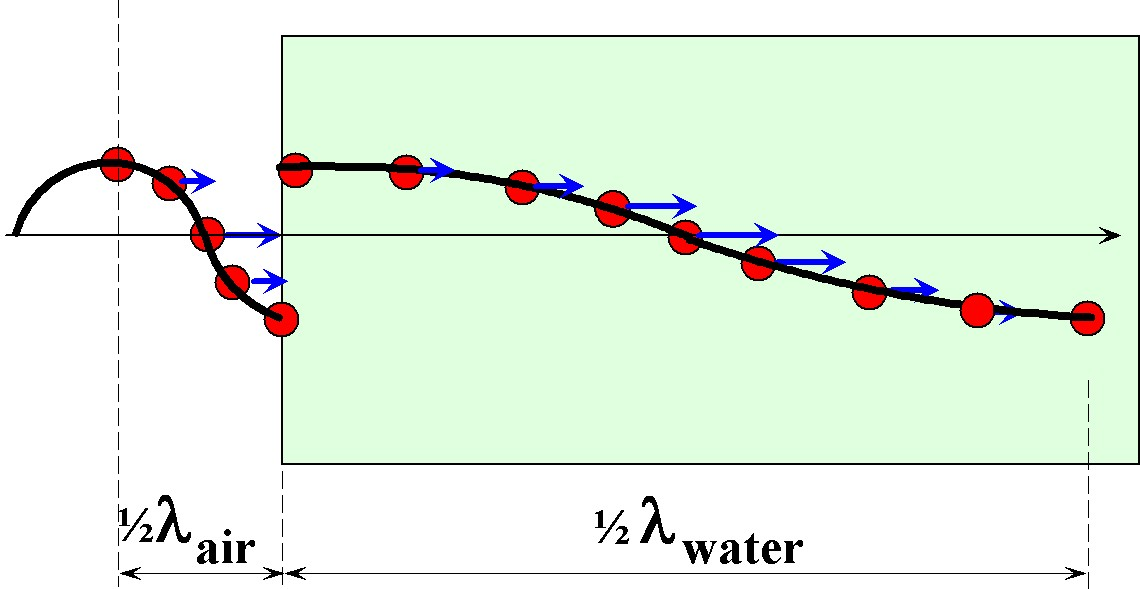
\includegraphics[width=5in]{./figures/Topic3/Fig3-6.jpg}
	\caption{A look at half a wavelength in media of different densities.}
 	\label{Fig3-6}
 \end{figure}
The mass propelled forward by the pressure spike can therefore be visualized as a rectangular volume with a length$1/2\lambda_a$ and a cross-sectional area $A_a$ perpendicular to the length. The mass of air $m_a$ is therefore 
\begin{equation}\label{eqn3-12}
m_a = \rho_a \frac{\lambda}{2}A_a
\end{equation}
Since the wavelength can be expressed in terms of speed of sound c and the frequency $f$ ($\lambda_a=c_a/f$), the mass $m_a$ can be expressed as 
\begin{equation}\label{eqn3-13}
m_a = \frac{\rho_a c_a A_a}{2f}
\end{equation}
Similarly, the mass of the water that the air collides with is 
\begin{equation}\label{eqn3-14}
m_w = \frac{\rho_w c_w A_w}{2f}
\end{equation}
where $A_w$ is the area of the water that is pushed.  
Substituting Eqs.~\ref{eqn3-13} and \ref{eqn3-14} into Eq.\ref{eqn3-11}, we see that 
\begin{equation}\label{eqn3-15}
T = \frac{4\rho_w c_w A_w/\rho_a c_a A_a}{\left(1+\rho_w c_w A_w/\rho_a c_a A_a\right)^2}
\end{equation}
What if the middle ear did not exist, that is, what if air waves struck the fluid in the inner ear directly?  Then $A_a$ would equal $A_w$.  Given that $\rho_w/\rho_a$ = 800/1 and $c_w/c_a$ = 5/1 when the medium $a$ is air and the medium $w$ is water,
$$T = \frac{4\cdot 800\cdot 5\cdot 1}{\left(1+800\cdot5\cdot1\right)^2} = 0.001$$
A 0.1\% transmission corresponds to a transmission level that is 1000 times smaller than the initial level. According to Eq.~\ref{eqn3-6}, the corresponding decibel change is
\begin{eqnarray}
{\rm dB~change} &=& 10 \log_{10}\left(\frac{I_{\rm final}}{I_{\rm initial}}\right)\nonumber\\
&=& 10 \log_{10}\frac{1}{1000}\nonumber\\
&=& -30~{\rm dB}\nonumber
\end{eqnarray}
or a loss of 30 decibels. This is the equivalent of a loud concert becoming a whisper.

The transmission can also be written in terms of impedance.  Recall Eq.~\ref{eqn3-4}, which states that impedance $\mathcal{Z} = \rho cA$.  Eq.~\ref{eqn3-11} becomes
\begin{equation}\label{eqn3-16}
T = \frac{4\mathcal{Z}_w/\mathcal{Z}_a}{\left(1+\mathcal{Z}_w/\mathcal{Z}_a\right)^2}
\end{equation}
Fig.~\ref{Fig3-7} plots how the transmission depends on the impedance ratio, according to Eq.~\ref{eqn3-16}.  To get 100\% transmission, $\mathcal{Z}_a$ must equal, or match, $\mathcal{Z}_w$.  This is why impedance matching is so important to maximize transmission.  
 \begin{figure}[h]
	\centering
	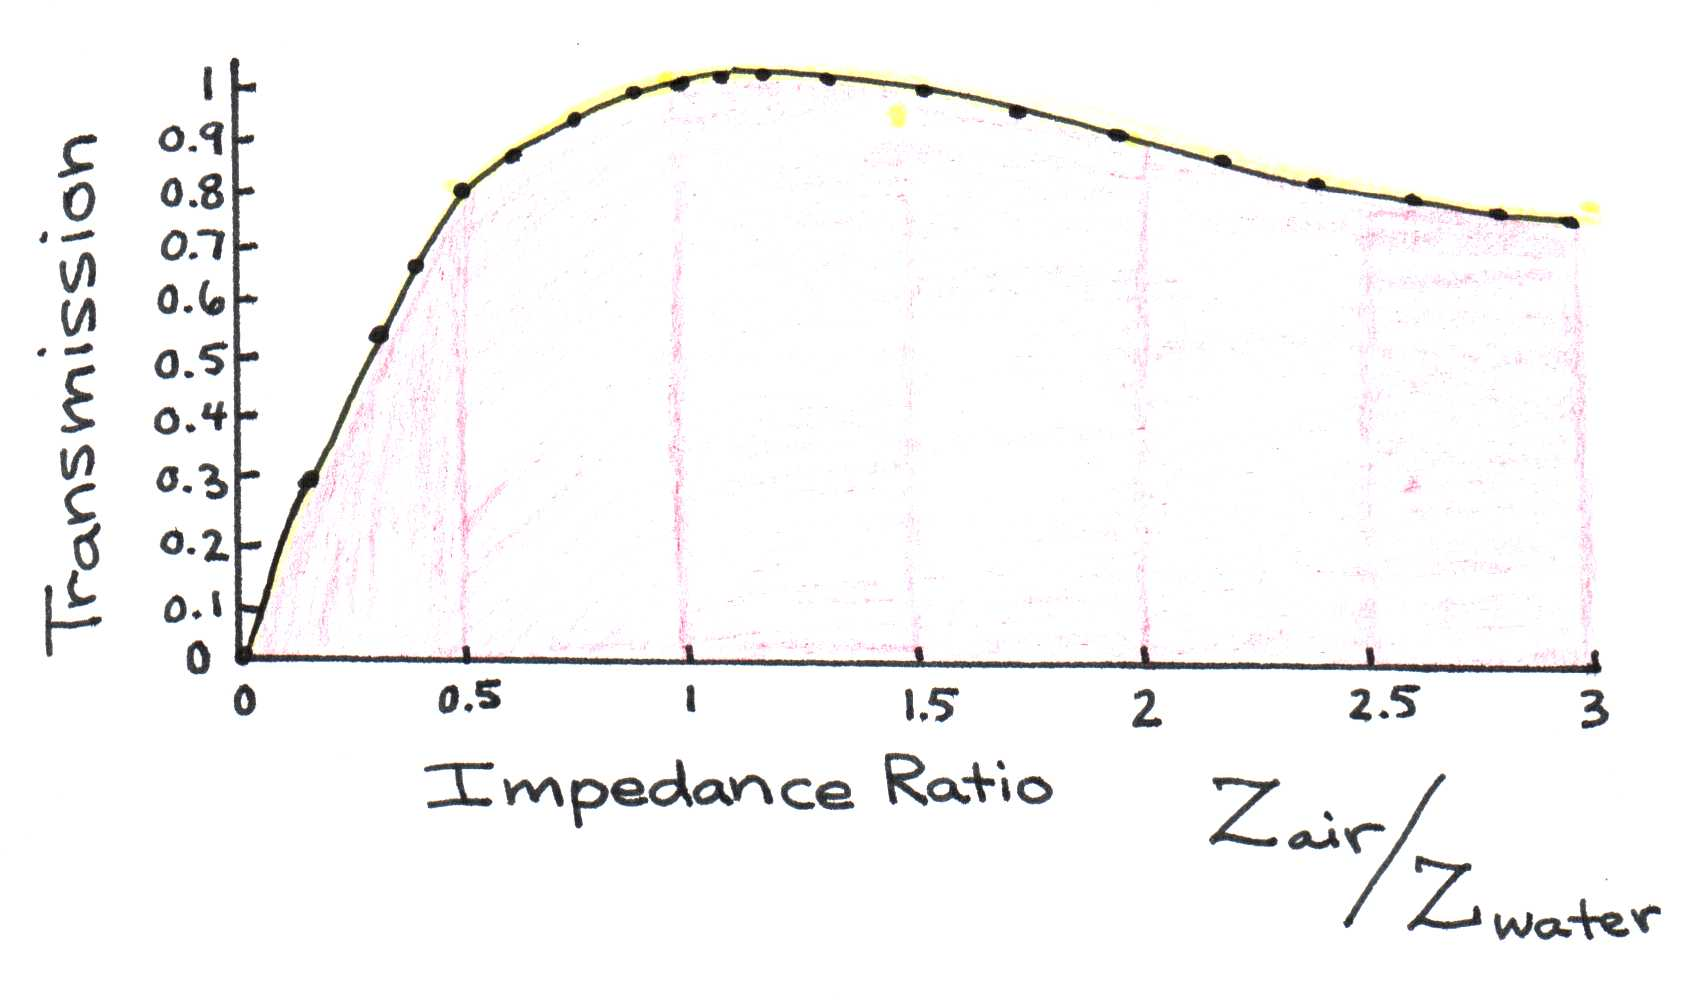
\includegraphics[width=5in]{./figures/Topic3/Fig3-7.jpg}
	\caption{Dependence of transmission on impedance ratio.  Note that transmission is 100\% effective only when the impedances are equal.}
 	\label{Fig3-7}
 \end{figure}  
So what would happen if the middle ear was not present, and sound waves struck directly the oval window of the fluid-filled inner ear? In that case the sound transmission would diminish by 30 decibels as our calculations predict. Fortunately, our hearing has evolved a way to minimize the impact of impedance mismatch at the interface between air and water. Sound waves traveling through air strike the surface $A_{eardrum}$ of the ear drum. This acoustical power is then channeled through the middle ear bones into a much smaller area focused around the oval window. The ratio of the areas $A_{eardrum}/A_{oval-window}$ results in a ratio $A_a/A_w\approx 20$ in Eq.~\ref{eqn3-14}, rather than 1 as we assumed without the middle ear. In terms of impedance, the mismatch between $\mathcal{Z}_a$ and $\mathcal{Z}_w$ ($\mathcal{Z}_a$/$\mathcal{Z}_w$ = 1/4000) is now significantly reduced ($\mathcal{Z}_a$/$\mathcal{Z}_w$ = 20/4000), allowing the sound transmission into the inner ear to increase approximately 20 fold.  The function of the middle ear is thus to aid in impedance matching. 

\subsection{The Inner Ear}

The part of the inner ear used in hearing is called the cochlea (Latin for ``snail shell'').  This complex structure contains a coiled set of tubes, the inner structure of which is shown in greater detail in Figure \ref{Fig3-8}.  
 \begin{figure}[htb]
	\centering
	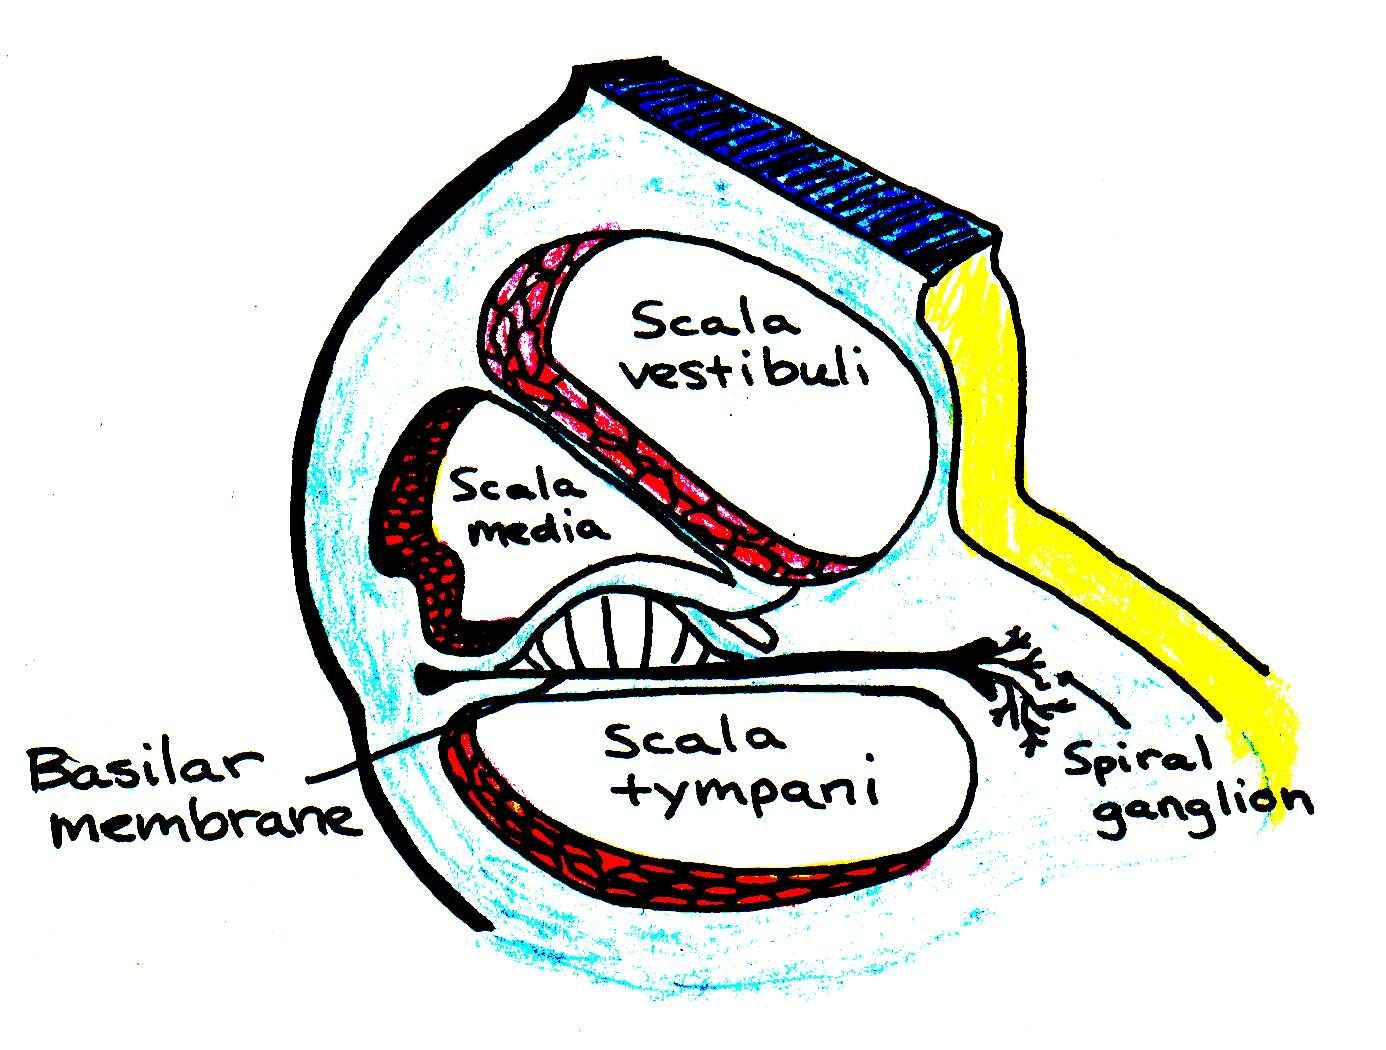
\includegraphics[width=5in]{./figures/Topic3/Fig3-8.jpg}
	\caption{Cross-section through one of the turns of the cochlea. }
 	\label{Fig3-8}
\end{figure}   
The conversion of acoustic signals to nerve impulses takes place in the cochlea, specifically at hair cells located in the space between the scala tympani and the scala vestibuli.  When the stapes (stirrup) cause the oval window to vibrate, a traveling pressure wave is created in the cochlear fluid.  The basilar membrane, which extends along the length of the cochlea, vibrates in response to the pressure wave.  
\begin{figure}[htb]
	\centering
	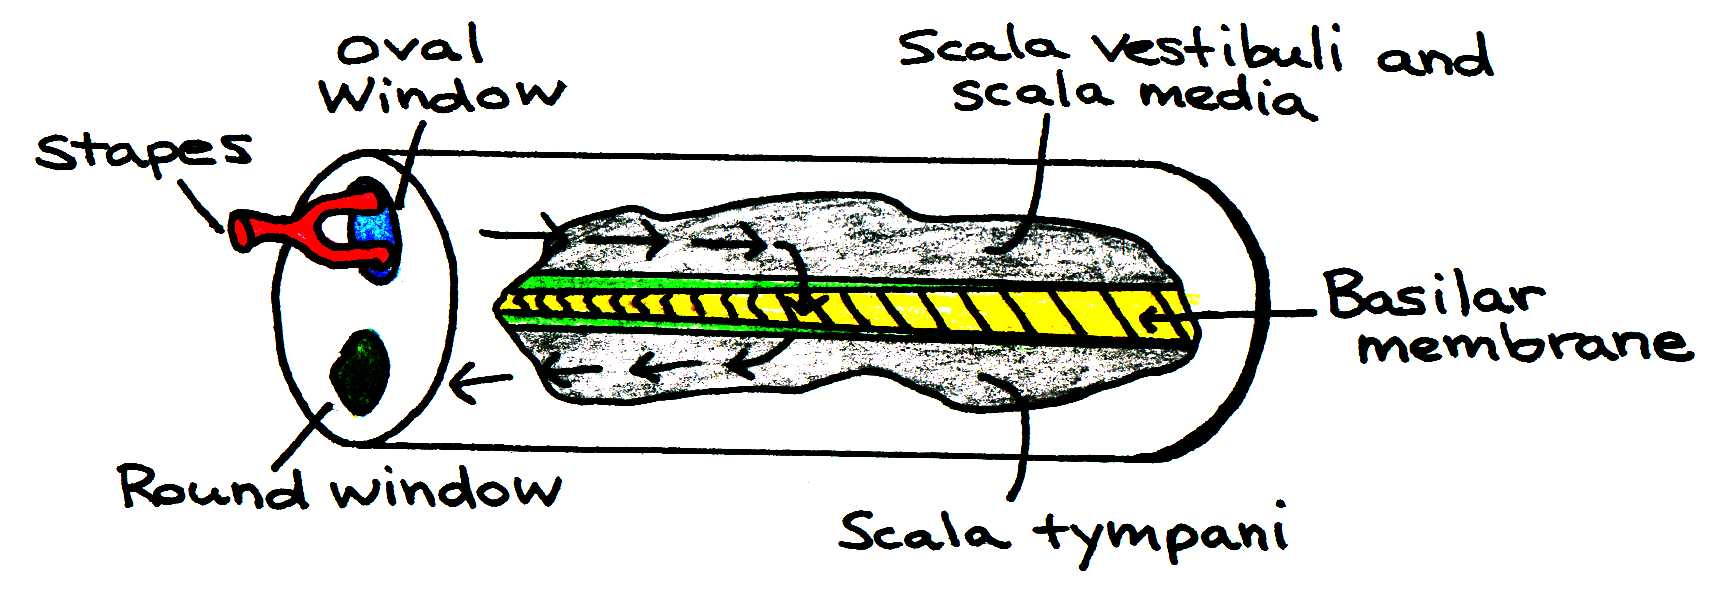
\includegraphics[width=\textwidth]{./figures/Topic3/Fig3-9.jpg}
	\caption{Movement of fluid in the cochlea.}
 	\label{Fig3-9}
\end{figure}
Basilar fibers, which vary in length and stiffness along the basilar membrane, respond to the wave by bending back and forth.  See Fig.~\ref{Fig3-10}. Movement of these fibers causes hair cells in the immediate vicinity to vibrate, which triggers nerve impulses that travel to the brain and are interpreted as a sound of a particular frequency. The function of the inner ear relies heavily on the resonance phenomenon. We will now model the physics of resonance in basilar fiber motion.  

\subsubsection{Resonance in Basilar Fiber Motion}

Consider a simple elastic system that is allowed to oscillate, as shown in Figure \ref{Fig3-10}, where $k$ is the elastic constant.  
 \begin{figure}[htb]
 	\centering
	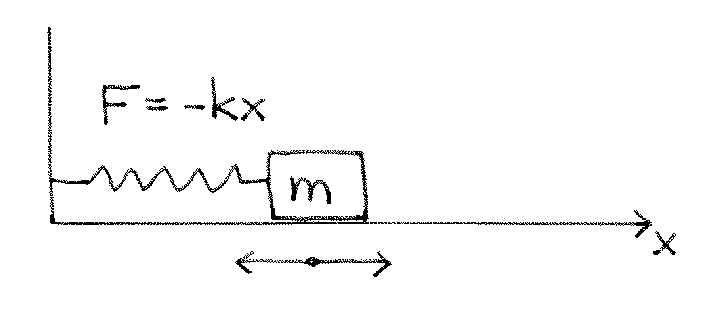
\includegraphics[width=5in]{./figures/Topic3/Fig3-10.jpg}
	\caption{A simple elastic system.}
 	\label{Fig3-10}
 \end{figure}
Applying Netwon’s 2nd law of motion,
\begin{eqnarray}\label{eqn3-17}
	\sum F_x &=& ma\nonumber\\
	-kx &=& m \frac{d^2x}{dt^2}\nonumber\\
	\frac{d^2x}{dt^2} &=& -\frac{k}{m}x 
\end{eqnarray}
This differential equation is very similar to the one obtained in the pendulum problem in Topic 1.  The solution to this equation is 
 \begin{equation}\label{eqn3-18}
	 x(t) = A \sin\left(\sqrt{\frac{k}{m}}t\right)
 \end{equation}
Letting $T\sqrt{k/m} = 2\pi$, we find that the period $T=2\pi\sqrt{m/k}$. The resonant frequency of the system associated with this vibration is therefore
$$f_{\circ}=\frac{1}{T} = \frac{1}{2\pi}\sqrt{\frac{k}{m}}$$

The basilar fibers in the inner ear behave like reeds.  Reeds vibrate with a certain frequency since they are free to oscillate.  They have a stiffness $k$ and some inertia $m$.  As mentioned before, the length of the basilar fibers is not uniform.  Near the stapes, they are 0.04 mm, increasing steadily with distance from the stapes to a length of 0.5 mm.  At the same time, the stiffness of the fibers decreases by a factor of 100.  Both of these factors contribute to a significant change in the ratio $k/m$, which affects the resonant frequency of the fibers.

The frequency of the incoming traveling wave determines how deep the wave penetrates the cochlea.  High-frequency waves resonate best at the short, stiff fibers near the stapes, so the sound is absorbed there.  Low-frequency waves travel much farther along the basilar membrane before being absorbed by the longer, more flexible fibers.  Figure \ref{Fig3-11} illustrates this fact.  
\begin{figure}[htb]
	\centering
 	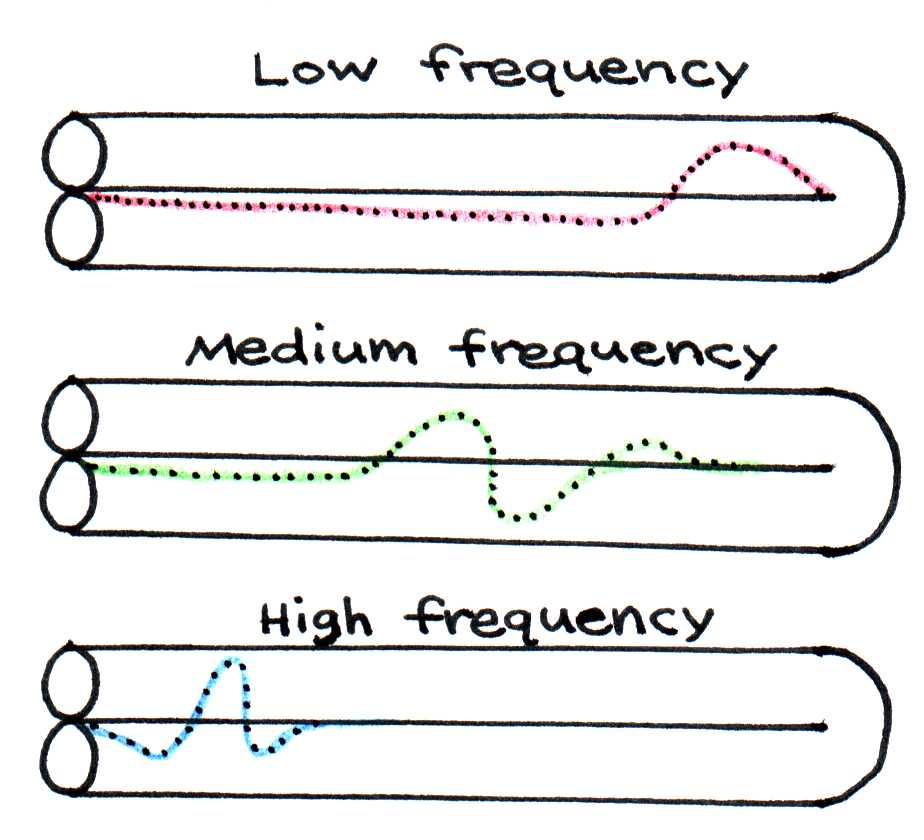
\includegraphics[width=4.5in]{./figures/Topic3/Fig3-11.jpg}
 	\caption{Traveling waves along the basilar membrane.}
	\label{Fig3-11}
\end{figure}
 
The basilar fibers allow us to distinguish the loudness and pitch of a sound.  A wave with a large amplitude causes the fibers to vibrate vigorously.  In response, action potentials are rapidly created, and the brain interprets this as a loud sound.  A sound wave with a high frequency, on the other hand, causes hair cells adjacent to a point on the basilar membrane near the oval window to vibrate.  This stimulates neurons to fire signals to the brain that are interpreted as a high pitch.